%%===========================================================%%
%%                                                           %%
%%                       EFFICIENCIES                        %%
%%                                                           %%
%%===========================================================%%


\chapter{Efficiencies}\label{chap:efficiencies}
\section{General overview}
It is the best to apply the corrections to the measured distributions  that are based on real data analysis. However, due to the complexity of the processes we are studying, it is necessary to obtain corrections from the MC simulation. Whenever possible, we compare efficiencies obtained from data with those from the MC and introduce appropriate corrections to the MC if necessary.

It is prefered to get the detector to true-level corrections from the MC, which is dedicated to the studied physics process. However, for this purpose, the~statistics in the MC should be several times greater (preferably an order of magnitude) than we have in the data for analysis. This is not possible with generally low total efficiency $\left(\textrm{TPC \& TOF \& RP}\right)$. On the other hand, such efficiencies depend on the modeling of the studied process and require a good description of all generally multidimensional distributions  by MC. Since that, the basic method of corrections that we use in the analyses is the method of factorization of global efficiency into the product of single-particle efficiencies (separate for each central particle and forward protons). Thereby,  statistically precise multidimensional corrections on TPC, TOF and RP are obtained. Nevertheless, this method does not correct on the migration effects caused by the finite detector resolution and is sensitive to the binning. Whenever possible, we use both methods of correction (at least in the consistency tests for MC samples). In this note, only the single-particle corrections are described, which are common for both analyses.

\section{TPC track acceptance and reconstruction efficiency}\label{sec:tpcAccAndEff}
We defined joint acceptance and efficiency of reconstruction of a track in the TPC, $\epsilon_{\textrm{\tiny TPC}}$, as the probability that particle from the primary interaction generates signal in the detector which is reconstructed as a global track that satisfies all quality criteria (cuts~\ref{sec:TpcQualityCuts}).
To derive this quantity the single particle STARsim MC embedded into zero-bias trigger data taken simultaneously with physics triggers 
 was used.
\subsection{STAR nominal method}
Technically, the common method used by the STAR to obtain  $\epsilon_{\textrm{\tiny TPC}}$ is the following procedure:
\begin{enumerate}
	\item True-level primary particles of given ID and charge were selected ($set~A$).
	\item Each particle from $set~A$ was checked if at least one global TPC track with more than half of hit points associated to it was generated by true-level particle  (definition of true level particle-track matching, idTruth from StMuTrack collection). All particles from $set~A$ which have associated global track satisfying quality criteria (cut~\ref{sec:TpcQualityCuts}) formed $set~B$.
	\item The joint TPC acceptance and efficiency was calculated as the ratio of the histograms of true level quantities (such as $p_{T}$, $\eta$, $z_{\textrm{vtx}}$) for particles from $set~B$ and particles from $set~A$:
	\begin{equation}\label{eq:tpcAccAndEffDefinition}
	\epsilon_{\textrm{\tiny TPC}}\left(p_{T}, \eta, z_{vtx};~\textrm{sign},\textrm{PID}\right) = \frac{(p_{T},\eta, z_{vtx})~\textrm{histogram for particles of given sign and ID from}~set~B}{(p_{T},\eta, z_{vtx})~\textrm{histogram for particles of given sign and ID from}~set~A}.
	\end{equation}
	
\end{enumerate}
\subsubsection{Global track to true level particle matching}
It was found during the analysis that in about $1\%$ events there are more than one reconstructed global track matched with the same true level particle, which is shown in Fig.~\ref{fig:trackSplittingNominal}, separatelly for true level pions, kaons and protons.
\begin{figure}[ht]
	\centering
	\parbox{0.329\textwidth}{
		\centering
		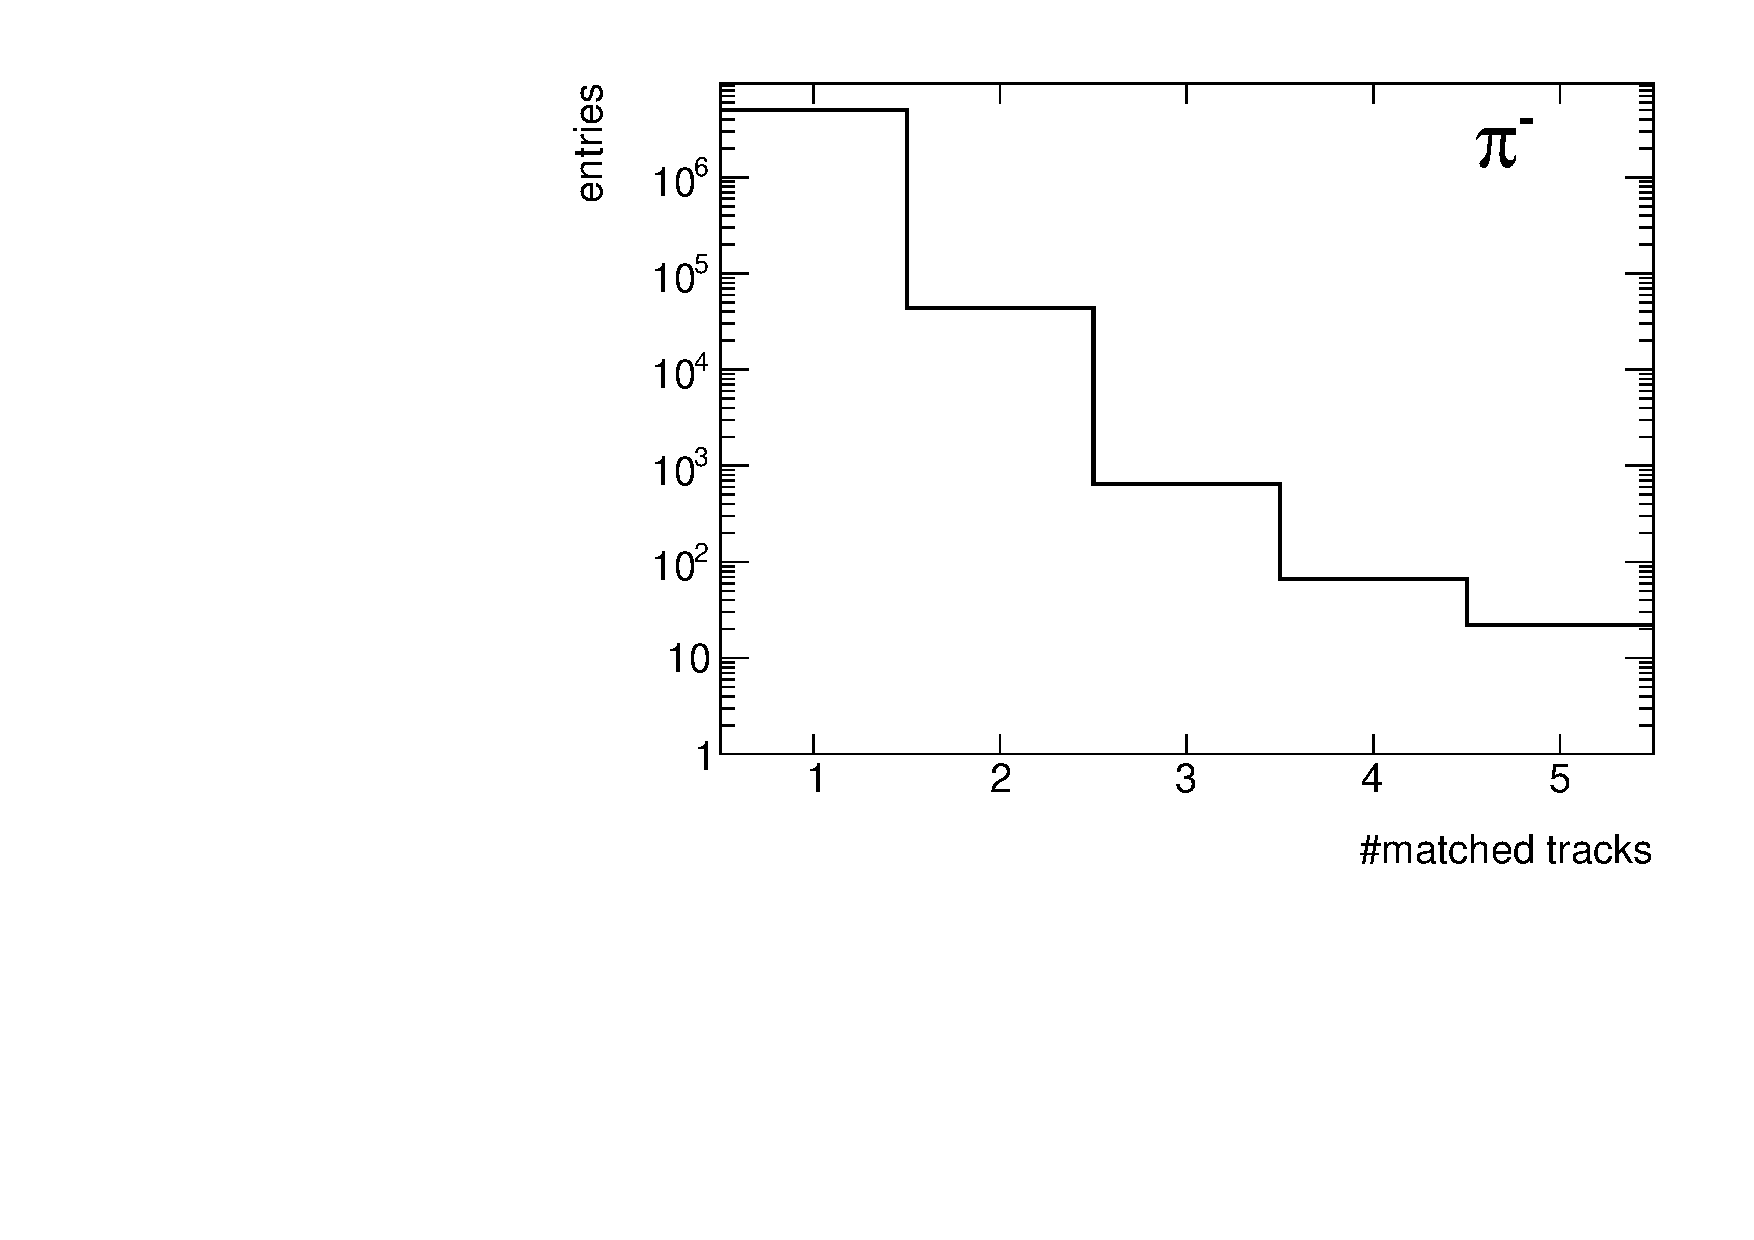
\includegraphics[width=\linewidth,page=1]{graphics/eff/trackSplitting_CD.pdf}\\
		\includegraphics[width=\linewidth,page=4]{graphics/eff/trackSplitting_CD.pdf}\\
	}~
	\parbox{0.329\textwidth}{
		\centering
		\includegraphics[width=\linewidth,page=2]{graphics/eff/trackSplitting_CD.pdf}\\
		\includegraphics[width=\linewidth,page=5]{graphics/eff/trackSplitting_CD.pdf}\\
	}%
	\parbox{0.329\textwidth}{
		\centering
		\includegraphics[width=\linewidth,page=3]{graphics/eff/trackSplitting_CD.pdf}\\
		\includegraphics[width=\linewidth,page=6]{graphics/eff/trackSplitting_CD.pdf}\\
	}%
	\caption[Number of reconstructed global tracks, satisfying all quality criteria, matched with the same true level primary particle.]{Number of reconstructed global tracks, satisfying all quality criteria (cuts~\ref{sec:TpcQualityCuts}), matched with the~same true level primary particle. The type of true level particle is indicated in the figure.}\label{fig:trackSplittingNominal}
\end{figure}

The true level particle end vertex $V_r^{end}$ is not specified if the particle neither interacted with the dead material nor decayed. The analysis showed that $1\%$ of the reconstructed tracks are matched to the true particle which lost identitiy ($V_r^{end}<48$~cm) before entering TPC. We interprate such situation as matching of reconstructed daugther particle to true level parent particle. It is potentially dangerous since  momentum and type of daugther particle might be different from parent particle.  Problem with wrong true level matching is also present for tracks with only one track matched to true level particle which do not decay or interact with material (no end vertex assosiated to true  level particle). 
It is visible on Fig.~\ref{fig:trackSplittingNominaldEdx} where $dE/dx$ is shown that some reconstracted tracks 
have different PID than true level particle matched to it.
 Also, there are problems in the closure tests, where  the  reconstructed-level distributions of rapidity and transverse momenta weighted by the nominal efficiency corrections do not describe the true level distributions. Main reason for failing of closure tests is non-negligible (and significant   for anti-protons) amount of global tracks matched with primary particles but no or little correlation in $\eta-\phi$ space beetwen
matched pair. 
The~distance 
\begin{equation}\label{eq:tpcMatchingDeltaSquare}
\delta^{2}\left(\eta,\phi\right)=\left(\eta^{true}-\eta^{reco}\right)^2+\left(\phi^{true}-\phi^{reco}\right)^2
\end{equation}
between the true level particle and global track assigned to it, shown in Fig.~\ref{fig:trackSplittingNominalDelta_1} for particles with only one  matched global track and Fig.~\ref{fig:trackSplittingNominalDelta_2} for particles with at least two  matched global tracks, indicates that some part of the tracks taken for the efficiency calculation are measured very badly ($\delta^{2}\left(\eta,\phi\right)$ is very large), even if there is only one global track matched to the true-particle.
\begin{figure}[ht]
	\centering
	\parbox{0.329\textwidth}{
		\centering
		\includegraphics[width=\linewidth,page=31]{graphics/eff/trackSplitting_CD.pdf}\\
		\includegraphics[width=\linewidth,page=34]{graphics/eff/trackSplitting_CD.pdf}\\
	}~
	\parbox{0.329\textwidth}{
		\centering
		\includegraphics[width=\linewidth,page=32]{graphics/eff/trackSplitting_CD.pdf}\\
		\includegraphics[width=\linewidth,page=35]{graphics/eff/trackSplitting_CD.pdf}\\
	}%
	\parbox{0.329\textwidth}{
		\centering
		\includegraphics[width=\linewidth,page=33]{graphics/eff/trackSplitting_CD.pdf}\\
		\includegraphics[width=\linewidth,page=36]{graphics/eff/trackSplitting_CD.pdf}\\
	}%
	\caption[$dE/dx$ of the track matched to true level particle.]{$dE/dx$ of the track matched to true level particle. Lines indicate Bichsel function prediction for each particle species. Only tracks matched to non-interacting true level particles without end vertex  are shown.}\label{fig:trackSplittingNominaldEdx}
\end{figure}

Because of several above mentioned  problems with  nominal STAR definition of matching between reconstructed tracks and true  level particles we decided to use in the analysis modified matching            
definition by taking into the account the difference    between reconstructed tracks and true particles in $\eta-\phi$ space.




\begin{figure}[hb]
	\centering
	\parbox{0.329\textwidth}{
		\centering
		\includegraphics[width=\linewidth,page=25]{graphics/eff/trackSplitting_CD.pdf}\\
		\includegraphics[width=\linewidth,page=28]{graphics/eff/trackSplitting_CD.pdf}\\
	}~
	\parbox{0.329\textwidth}{
		\centering
		\includegraphics[width=\linewidth,page=26]{graphics/eff/trackSplitting_CD.pdf}\\
		\includegraphics[width=\linewidth,page=29]{graphics/eff/trackSplitting_CD.pdf}\\
	}%
	\parbox{0.329\textwidth}{
		\centering
		\includegraphics[width=\linewidth,page=27]{graphics/eff/trackSplitting_CD.pdf}\\
		\includegraphics[width=\linewidth,page=30]{graphics/eff/trackSplitting_CD.pdf}\\
	}%
	\caption[$\delta^{2}\left(\eta,\phi\right)$ distributions between true level particles and tracks assigned to them.]{$\delta^{2}\left(\eta,\phi\right)$ distributions  between true level particles and tracks assigned to them. Only true level particles with only one reconstructed track matched to them were selected. Red lines and arrows indicate  the~cut value of $0.15^2$, which is used in the modified true level particle-track matching definition.}\label{fig:trackSplittingNominalDelta_1}
\end{figure}

\begin{figure}[h!]\vspace{-10pt}
	\centering
	\parbox{0.329\textwidth}{
		\centering
		\includegraphics[width=\linewidth,page=19]{graphics/eff/trackSplitting_CD.pdf}\\
		\includegraphics[width=\linewidth,page=22]{graphics/eff/trackSplitting_CD.pdf}\\
	}~
	\parbox{0.329\textwidth}{
		\centering
		\includegraphics[width=\linewidth,page=20]{graphics/eff/trackSplitting_CD.pdf}\\
		\includegraphics[width=\linewidth,page=23]{graphics/eff/trackSplitting_CD.pdf}\\
	}%
	\parbox{0.329\textwidth}{
		\centering
		\includegraphics[width=\linewidth,page=21]{graphics/eff/trackSplitting_CD.pdf}\\
		\includegraphics[width=\linewidth,page=24]{graphics/eff/trackSplitting_CD.pdf}\\
	}%
	\caption[$\delta^{2}\left(\eta,\phi\right)$ distributions between true level particles and tracks assigned to them.]{$\delta^{2}\left(\eta,\phi\right)$ distributions between true level particles and tracks assigned to them. Only true level particles with at least two reconstructed tracks matched to them were selected. Red lines and arrows indicate  the~cut value of $0.15^2$, which is used in the modified true level particle-track matching definition.}\label{fig:trackSplittingNominalDelta_2}
\end{figure}




\subsection{Method used in this analysis}\label{subsec:definitionTrueLevelMatching}
In this method, the definition of true level particle-track matching is modified. In addition to the requirement of the appropriate number of common hit points, the distance between true level particle and track is required to be smaller than $0.15$, $\delta^{2}\left(\eta,\phi\right)<\left(0.15\right)^2$. It is quite an arbitrary value which should be small but not too small  to loose good events. The value of $\delta^2$ cut was chosen by the requirement that only acceptable small amount of CEP events which passed all selection criteria will not satisfy matching criteria. It was verified with the CEP MC embedded into zero-bias triggers that with quoted value of cut on $\delta^{2}\left(\eta,\phi\right)$ less than $0.3\%$ of CEP events have at least one track which is not considered to be matched with true-level pion despite the standard matching (Fig.~\ref{fig:deltaSqCEP}). We consider this an acceptably low effect.

Tracks, which do not satisfy the above criterion, are treated as fake tracks (even if they are matched to the true level particle in the standard way). In almost all cases, where the $\delta^{2}\left(\eta,\phi\right)<\left(0.15\right)^2$, there is only one track matched to true level particle (Fig.~\ref{fig:trackSplittingetaPhi}). Additionally, the $dE/dx$ of the track is mostly consistent with the true level PID (Fig.~\ref{fig:trackSplittingEtaPhidEdx}). Figure~\ref{fig:trackTPCefficiencyComparisonEtaPhi} shows the difference between TPC efficiencies obtained with the STAR standard and the modified definition of true particle-track matching.


%---------------------------
\begin{figure}[h!]%\vspace{-10pt}
	\centering
	\parbox{0.685\textwidth}{
		\centering
		\begin{subfigure}[b]{\linewidth}
			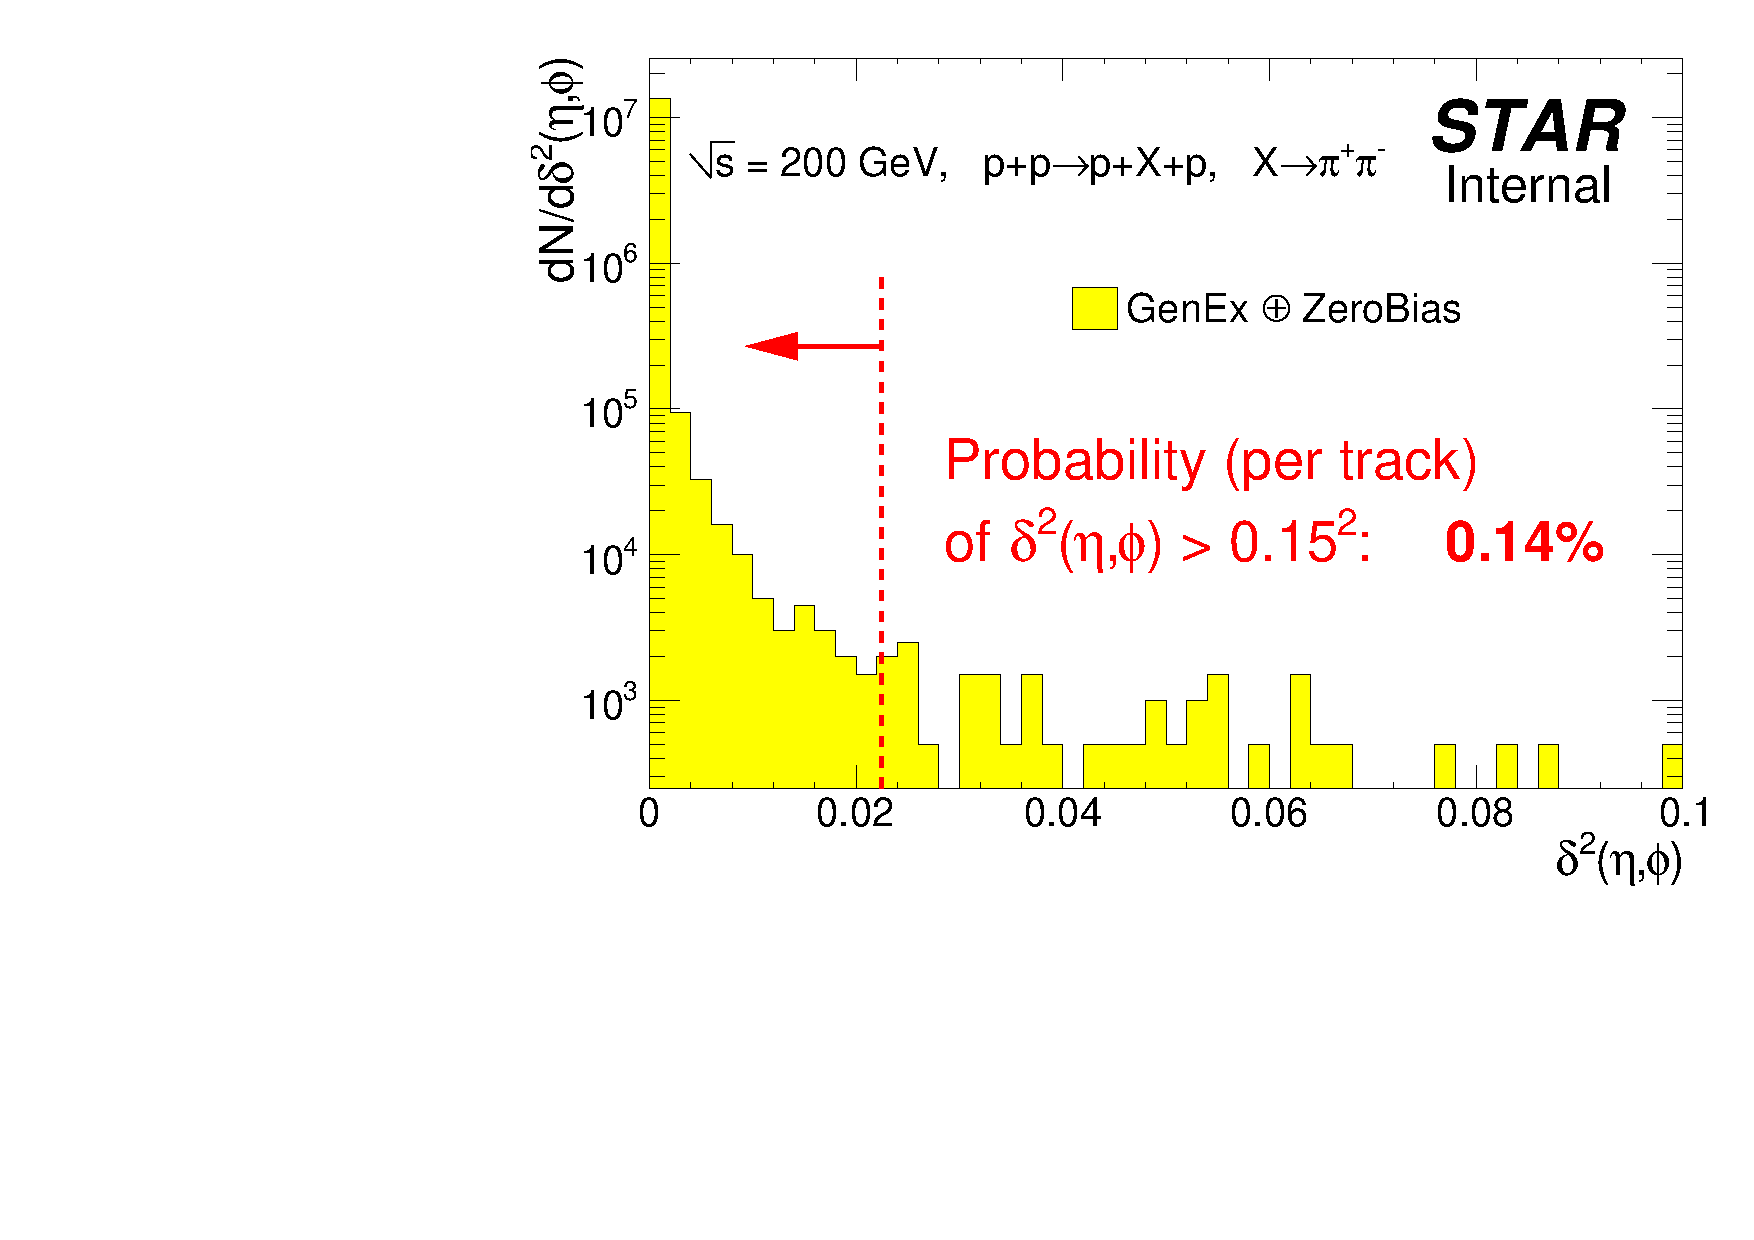
\includegraphics[width=\linewidth]{graphics/eff/deltaEtaSqDeltaPhiSqMatchedExclusive.pdf}
		\end{subfigure}
	}%
	\quad%
	\parbox{0.285\textwidth}{
		\centering
		\begin{minipage}[t][0.78\linewidth][t]{\linewidth}\vspace{-60pt}
			\caption[Distribution of $\delta^{2}\left(\eta,\phi\right)$ in CEP MC.]%
			{Distribution of $\delta^{2}\left(\eta,\phi\right)$ for tracks matched with true-level pions (using standard matching) in CEP MC embedded into zero-bias triggers. Tracks were taken from events passing full CEP event selection, recognized as exclusive $\pi^{+}\pi^{-}$. The vertical red dashed line indicates the cut value of $0.15^{2} \approx 0.023$, above which less than 0.14\% of tracks is contained.}%
			\label{fig:deltaSqCEP}
		\end{minipage}
	}
\end{figure}
%---------------------------


\begin{figure}[ht]
	\centering
	\parbox{0.329\textwidth}{
		\centering
		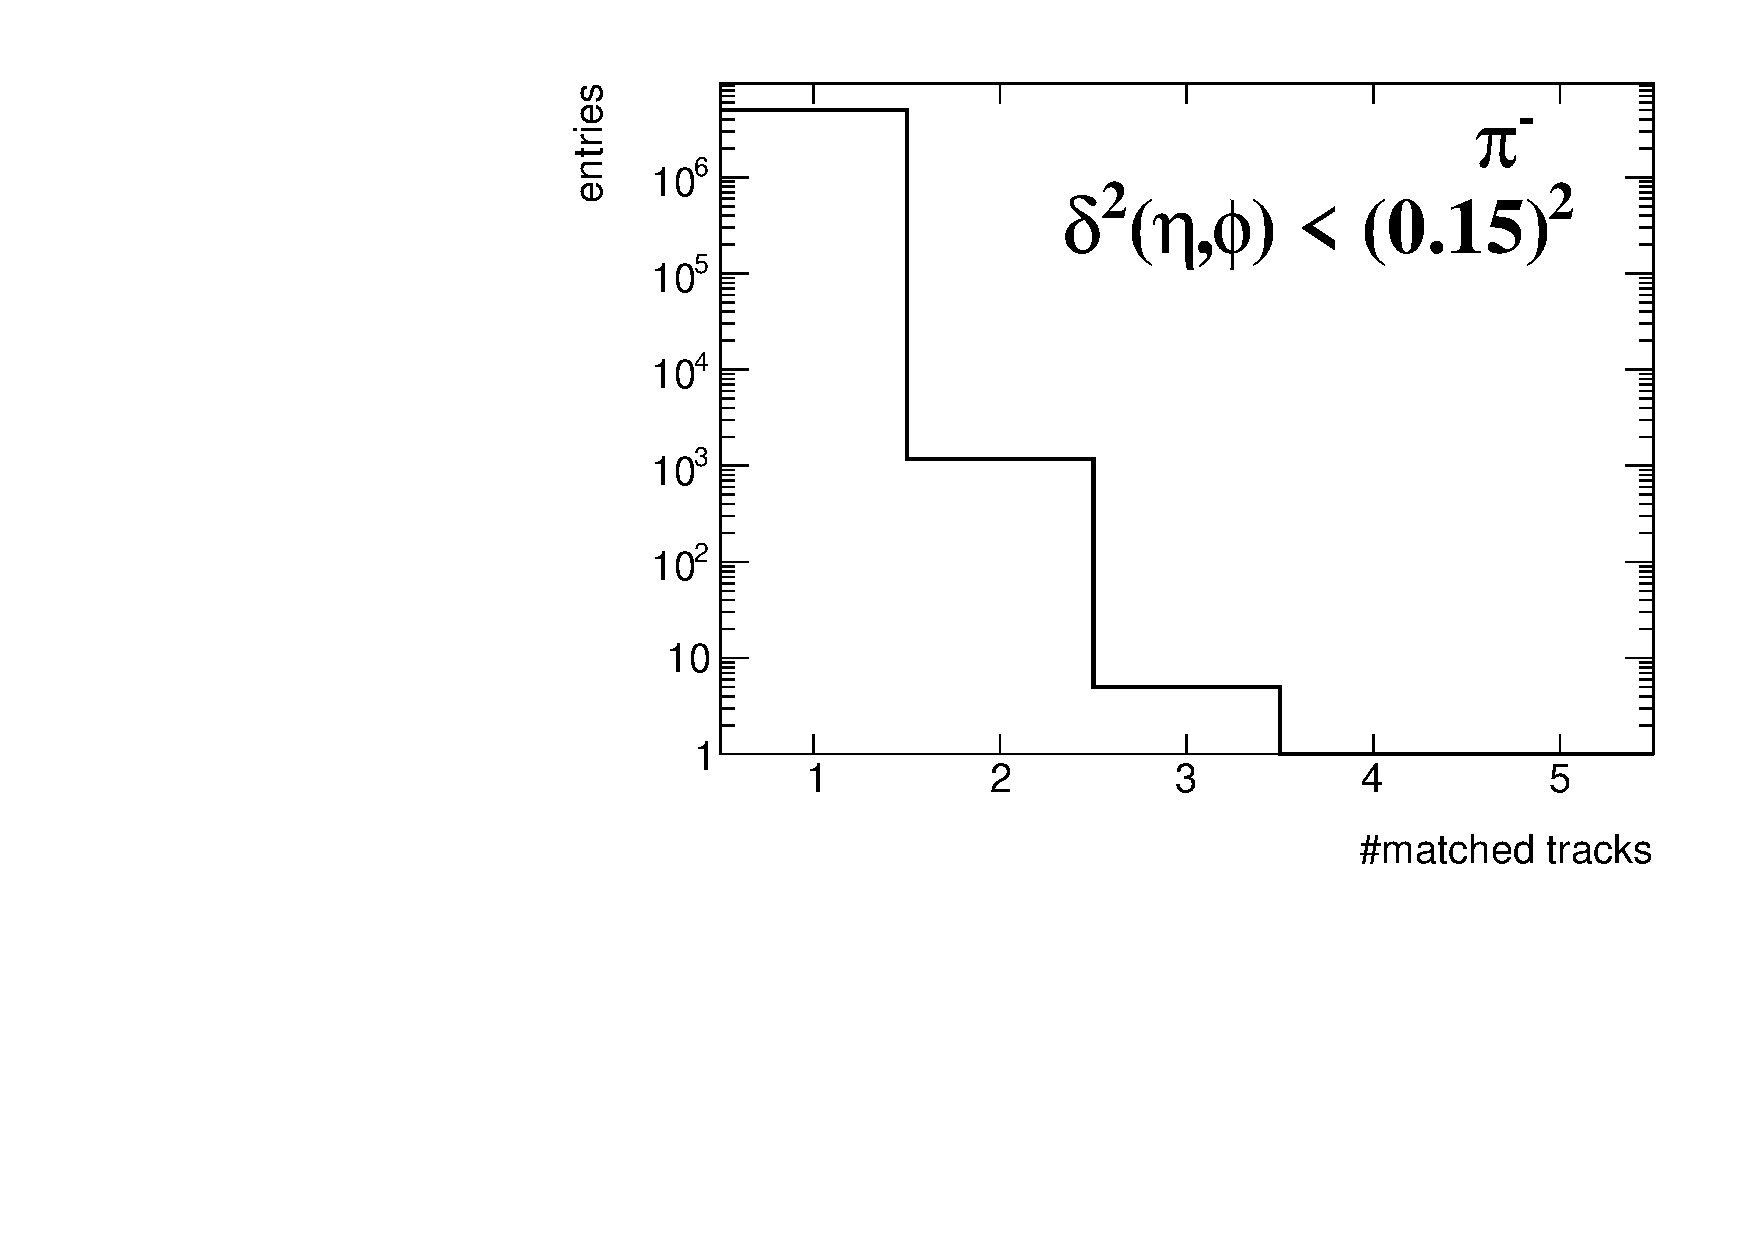
\includegraphics[width=\linewidth,page=1]{graphics/eff/trackSplitting_QualityEtaPhiCD.pdf}\\
		\includegraphics[width=\linewidth,page=4]{graphics/eff/trackSplitting_QualityEtaPhiCD.pdf}\\
	}~
	\parbox{0.329\textwidth}{
		\centering
		\includegraphics[width=\linewidth,page=2]{graphics/eff/trackSplitting_QualityEtaPhiCD.pdf}\\
		\includegraphics[width=\linewidth,page=5]{graphics/eff/trackSplitting_QualityEtaPhiCD.pdf}\\
	}%
	\parbox{0.329\textwidth}{
		\centering
		\includegraphics[width=\linewidth,page=3]{graphics/eff/trackSplitting_QualityEtaPhiCD.pdf}\\
		\includegraphics[width=\linewidth,page=6]{graphics/eff/trackSplitting_QualityEtaPhiCD.pdf}\\
	}%
	\caption[Number of reconstructed global tracks, satisfying all quality criteria and $\delta^{2}\left(\eta,\phi\right)$ cut, matched with the same true level primary particle.]{Number of reconstructed global tracks, satisfying all quality criteria (cuts~\ref{sec:TpcQualityCuts}) and $\delta^{2}\left(\eta,\phi\right)$ cut, matched with the same true level primary particle.}\label{fig:trackSplittingetaPhi}
\end{figure}


\begin{figure}[h!]%\vspace{-5pt}
	\centering
	\parbox{0.329\textwidth}{
		\centering
		\includegraphics[width=\linewidth,page=21]{graphics/eff/trackSplitting_QualityEtaPhiCD.pdf}\\
		\includegraphics[width=\linewidth,page=24]{graphics/eff/trackSplitting_QualityEtaPhiCD.pdf}\\
	}~
	\parbox{0.329\textwidth}{
		\centering
		\includegraphics[width=\linewidth,page=22]{graphics/eff/trackSplitting_QualityEtaPhiCD.pdf}\\
		\includegraphics[width=\linewidth,page=25]{graphics/eff/trackSplitting_QualityEtaPhiCD.pdf}\\
	}%
	\parbox{0.329\textwidth}{
		\centering
		\includegraphics[width=\linewidth,page=23]{graphics/eff/trackSplitting_QualityEtaPhiCD.pdf}\\
		\includegraphics[width=\linewidth,page=26]{graphics/eff/trackSplitting_QualityEtaPhiCD.pdf}\\
	}%
	\caption[$dE/dx$ of the closest track matched to true level particle passing the $\delta^{2}\left(\eta,\phi\right)$ cut.]{$dE/dx$ of the closest track matched to true level particle passing the $\delta^{2}\left(\eta,\phi\right)$ cut. Lines indicate Bichsel function prediction for each particle species.}\label{fig:trackSplittingEtaPhidEdx}
\end{figure}

\begin{figure}[ht]%[hb]
	\centering
	\parbox{0.329\textwidth}{
		\centering
		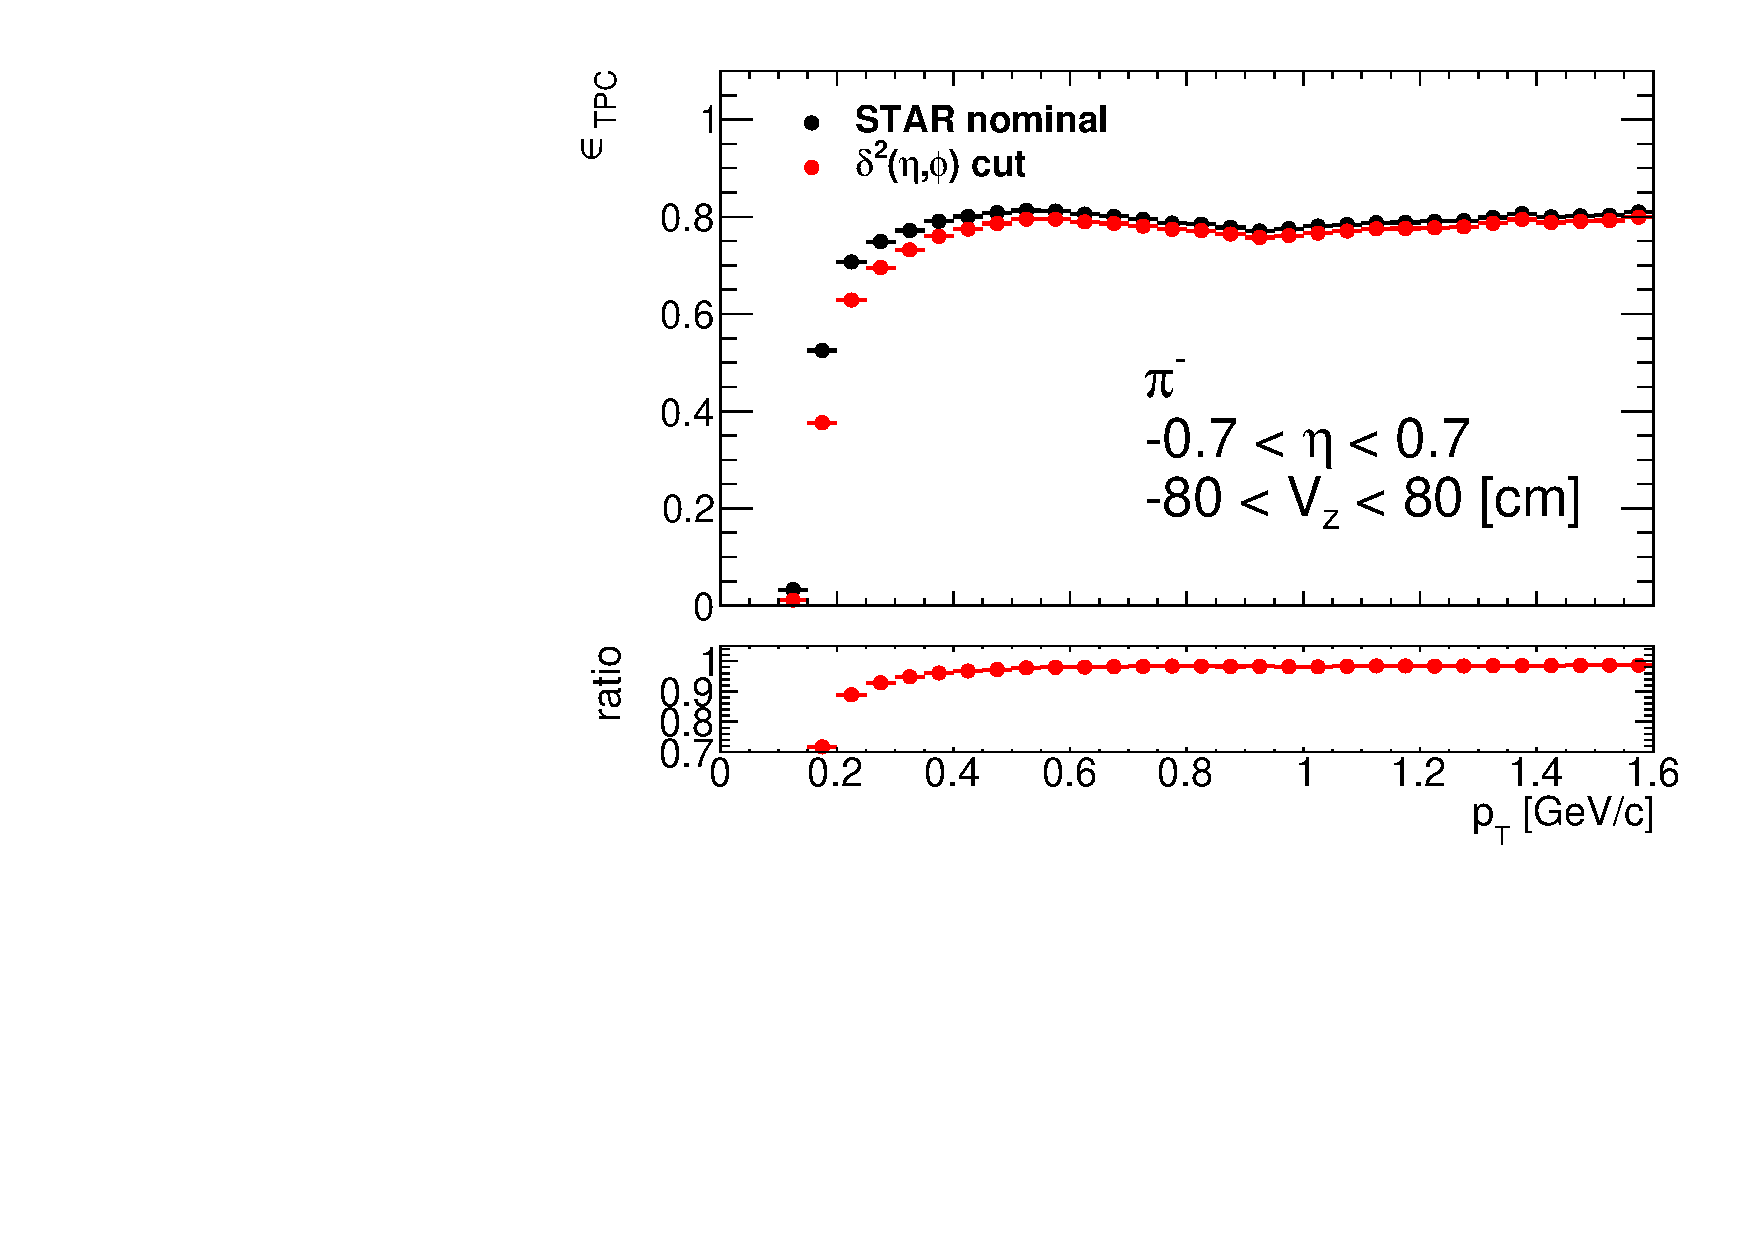
\includegraphics[width=\linewidth,page=1]{graphics/eff/tpcEffi.pdf}\\
		\includegraphics[width=\linewidth,page=4]{graphics/eff/tpcEffi.pdf}\\
	}~
	\parbox{0.329\textwidth}{
		\centering
		\includegraphics[width=\linewidth,page=2]{graphics/eff/tpcEffi.pdf}\\
		\includegraphics[width=\linewidth,page=5]{graphics/eff/tpcEffi.pdf}\\
	}%
	\parbox{0.329\textwidth}{
		\centering
		\includegraphics[width=\linewidth,page=3]{graphics/eff/tpcEffi.pdf}\\
		\includegraphics[width=\linewidth,page=6]{graphics/eff/tpcEffi.pdf}\\
	}%
	\caption[TPC acceptance and reconstruction efficiency as a function of $p_T$ $\left(|V_z|<80\textrm{ cm}, |\eta|<0.7\right)$ obtained from two methods.]{TPC acceptance and reconstruction efficiency as a function of $p_T$ $\left(|V_z|<80\textrm{ cm}, |\eta|<0.7\right)$ obtained from two methods.}\label{fig:trackTPCefficiencyComparisonEtaPhi}
\end{figure}


\subsection{Sample of  efficiency plots}\label{subsec:sampleTpcEffPlots}

In Figure~\ref{fig:tpcEff_pion_sample} we present sample plots of the TPC track and reconstruction efficiency calculated with modified definition of reconstructed track and true-level particle matching (according to description in Sec.~\ref{subsec:definitionTrueLevelMatching}), used in our analyses. Plots for all analyzed particle types and all bins of true $z_{\text{vtx}}$ are contained in Appendix~\ref{appendix:tpcEff}.

In order to maximize the statistics available for the measurement (possibly wide range of accepted longitudinal vertex position $z_{\text{vtx}}$) with maximized probed phase-space in analyzed physics processes (wide range of track $p_{T}$ and $\eta$) and minimized systematic uncertainties related to the central detector (TPC and TOF), we have studied the efficiency plots like ones shown in Fig.~\ref{fig:tpcEff_pion_sample} and Fig.~\ref{fig:tofEff_pion_sample}. We thus decided to set the cut on $z_{\text{vtx}}$ at $\pm80~\text{cm}$, which corresponds to 89\% of the full integral of normal distribution with mean at 0 and standard deviation of 50~cm. At the same time we set the cuts on track $p_{T}$ and $\eta$ as listed in Sec.~\ref{sec:TpcKinematicCuts}. These cuts are represented with red dashed lines in Fig.~\ref{fig:tpcEff_pion_sample} and Fig.~\ref{fig:tofEff_pion_sample}. Our goal was to operate within cuboid ($z_{\text{vtx}}$, $p_{T}$, $\eta$) region of relatively high TPC and TOF efficiency ($\geq50\%$ of the maximum value). In other words, we required high acceptance and efficiency for a rectangular ($p_{T}$, $\eta$) space with limits independent from $z_{\text{vtx}}$. One can see that the red lines in Fig.~\ref{fig:tpcEff_pion_sample} and Fig.~\ref{fig:tofEff_pion_sample} always contain in their interior the region of relatively high acceptance.

%---------------------------
\begin{figure}[h!]%\vspace{-10pt}
	\centering
	\parbox{0.485\textwidth}{
		\centering
		\begin{subfigure}[b]{\linewidth}
			\subcaptionbox{\label{fig:tpcEff_pion_sample_a}}{\includegraphics[width=\linewidth,page=3]{graphics/eff/Eff2D_TPC_pion_Minus.pdf}\vspace*{-8pt}}
		\end{subfigure}\\[5pt]
		\begin{subfigure}[b]{\linewidth}\addtocounter{subfigure}{1}
			\subcaptionbox{\label{fig:tpcEff_pion_sample_c}}{\includegraphics[width=\linewidth,page=18]{graphics/eff/Eff2D_TPC_pion_Minus.pdf}\vspace*{-8pt}}
		\end{subfigure}
	}%
	\quad%
	\parbox{0.485\textwidth}{
		\centering
		\begin{subfigure}[b]{\linewidth}\addtocounter{subfigure}{-2}
			\subcaptionbox{\label{fig:tpcEff_pion_sample_b}}{\includegraphics[width=\linewidth,page=11]{graphics/eff/Eff2D_TPC_pion_Minus.pdf}\vspace*{-8pt}}
		\end{subfigure}\\[5pt]
		\begin{minipage}[t][0.78\linewidth][t]{\linewidth}\vspace{10pt}
		\caption[Sample TPC acceptance and reconstruction efficiency of $\pi^{-}$.]{Sample TPC acceptance and reconstruction efficiency of $\pi^{-}$ in 3 bins of true $z_{\text{vtx}}$. Plots represents the TPC efficiency $\epsilon_{\text{TPC}}$ ($z$-axis) as a function of true particle pseudorapidity $\eta$ ($x$-axis) and transverse momentum $p_{T}$ ($y$-axis) in single $z$-vertex bin whose range is given at the top. Red lines and arrows indicate region accepted in analyses.}\label{fig:tpcEff_pion_sample}
		\end{minipage}
	}
\end{figure}
%---------------------------





\section{TOF acceptance, hit reconstruction and track matching efficiency}\label{sec:tofMatchEff}

Combined TOF acceptance, hit reconstruction efficiency and matching efficiency with TPC tracks, $\epsilon_{\textrm{\tiny TOF}}$, was defined as the probability that the global TPC track that satisfy quality criteria (cuts~\ref{sec:TpcQualityCuts}) is matched with hit in TOF (\ref{sec:TpcTofMatchingRequirement}). This quantity is generally referred as ``TOF efficiency''.

It was calculated in the very similiar way to TPC efficiency - single particle STARsim MC embedded into zero-bias triggers was used. Tracks belonging to $set~B$ from Sec.~\ref{sec:tpcAccAndEff} were utilized. From these tracks a sub-sample of tracks with non-zero TOF matching flag (StMuBTofPidTraits.mMatchFlag $>0$) was extracted ($set~C$). The TOF efficiency was calculated as
\begin{equation}\label{eq:tofAccAndEffDefinition}
		\epsilon_{\textrm{\tiny TOF}}\left(p_{T}, \eta, z_{vtx};~\textrm{sign},\textrm{PID}\right) = \frac{(p_{T},\eta, z_{vtx})~\textrm{histogram for particles of given sign and ID from}~set~C}{(p_{T},\eta, z_{vtx})~\textrm{histogram for particles of given sign and ID from}~set~B}.
	\end{equation}

An additional note has to be made here about the correction which is applied to TOF matching flag in MC analysis. It was found that in embedded simulation the dead TOF elements were not masked. To correct for this effect (hence obtain more reliable TOF efficiency) a data-based map of modules was created, separately for each RHIC fill. Map was filled with modules which were matched with TPC tracks in the data. In all MC sample analyses (including efficiency determination) each TPC track with non-zero TOF match flag was additionally checked if TOF module that track was matched with had any entries in the data-based map. If not - the TOF match flag was considered 0.

\subsection{Sample of  efficiency plots}

The sample TOF efficiency plot is shown in Fig.~\ref{fig:tofEff_pion_sample}. All remaining TOF efficiency plots are contained in Appendix~\ref{appendix:tofEff}.

%---------------------------
\begin{figure}[h!]%\vspace{-10pt}
	\centering
	\parbox{0.485\textwidth}{
		\centering
		\begin{subfigure}[b]{\linewidth}
			\subcaptionbox{\label{fig:tofEff_pion_sample_a}}{\includegraphics[width=\linewidth,page=3]{graphics/eff/Eff2D_TOF_pion_Minus.pdf}\vspace*{-8pt}}
		\end{subfigure}\\[5pt]
		\begin{subfigure}[b]{\linewidth}\addtocounter{subfigure}{1}
			\subcaptionbox{\label{fig:tofEff_pion_sample_c}}{\includegraphics[width=\linewidth,page=18]{graphics/eff/Eff2D_TOF_pion_Minus.pdf}\vspace*{-8pt}}
		\end{subfigure}
	}%
	\quad%
	\parbox{0.485\textwidth}{
		\centering
		\begin{subfigure}[b]{\linewidth}\addtocounter{subfigure}{-2}
			\subcaptionbox{\label{fig:tofEff_pion_sample_b}}{\includegraphics[width=\linewidth,page=11]{graphics/eff/Eff2D_TOF_pion_Minus.pdf}\vspace*{-8pt}}
		\end{subfigure}\\[5pt]
		\begin{minipage}[t][0.78\linewidth][t]{\linewidth}\vspace{10pt}
			\caption[Sample plotz of TOF acceptance, reconstruction and matching efficiency of $\pi^{-}$.]{Sample TOF acceptance, reconstruction and matching efficiency of $\pi^{-}$ in 3 bins of true $z_{\text{vtx}}$. Plots represents the TOF efficiency $\epsilon_{\text{TOF}}$ ($z$-axis) as a function of true particle pseudorapidity $\eta$ ($x$-axis) and transverse momentum $p_{T}$ ($y$-axis) in single $z$-vertex bin whose range is given at the top. Red lines and arrows indicate region accepted in analyses.}\label{fig:tofEff_pion_sample}
		\end{minipage}
	}
\end{figure}
%---------------------------

%---------------------------
%\begin{figure}[hb]%
%\centering\includegraphics[width=0.7\linewidth,page=11]{graphics/eff/Eff2D_TOF_pion_Minus.pdf}%
%\caption[Sample plot of TOF acceptance, reconstruction and matching efficiency of $\pi^{-}$.]{Sample plot of TOF acceptance, reconstruction and matching efficiency of $\pi^{-}$. Plot represents the TOF efficiency $\epsilon_{\text{TOF}}$ ($z$-axis) as a function of true particle pseudorapidity $\eta$ ($x$-axis) and transverse momentum $p_{T}$ ($y$-axis) in single $z$-vertex bin whose range is given at the top. Red lines and arrows indicate region accepted in analyses.}\label{fig:tofEff_pion_sample}
%\end{figure}
%---------------------------

As shown in Sec.~\ref{subsec:tofAbsEffSystAndCorr}, it was found during estimation of the systematic uncertainty of the TOF efficiency that the data-driven efficiency and MC effficiency (obtained with a method described in this section) differ significantly. Therefore the final TOF efficiency which is used to correct the data is a modified MC efficiency. Form of MC efficiency modification is given in ... .

% 
% \section{TPC vertex reconstruction efficiency}\label{sec:tpcVxRecoEff}
% 
% The definition of vertex reconstruction efficiency established in this analysis is the probability that two global tracks, both associated with true level primary particles from the kinematic region of the measurement, both satisfying kinematic and quality criteria (cuts~\ref{sec:TpcKinematicCuts} and ~\ref{sec:TpcQualityCuts}) and both matched with hits in TOF, form a vertex listed in the collection of reconstructed primary vertices and DCA(R) and DCA(z) of both global tracks calculated w.r.t. this vertex is contained within the limits of cut~\ref{sec:TpcDcaCuts}.
